\scanpage{33}

\deleted{\unsure{Les inclusions}}

on a \uline{loc}. des hom
\[
{}_nA\unsure{\longrightarrow|\mathbin{-}} A,\qquad{}_nA'\unsure{\longrightarrow|\mathbin{-}} A'
\]
d'où \uline{loc} \unsure{des hom}
\diagram{\begin{tikzcd}[
ampersand replacement=\&,column sep=large,row sep=large,
execute at end picture={
\draw[gray,line width=0.3pt]
([xshift=-5pt,yshift=4pt]\tikzcdmatrixname-2-2.west)
-- ([xshift=-1pt,yshift=-1pt]\tikzcdmatrixname-2-2.west)
-- ([xshift=-7pt,yshift=-4pt]\tikzcdmatrixname-2-2.west);
}]
\operatorname{Ext}^1(A\mathbin{\overset{L}{\otimes}}A\unsure{'},G_m)
\arrow[r]
\arrow[dr,start anchor=south east,end anchor=west,shorten >=5pt,bend right=6,
dash pattern=on 7mm off 3mm on 40mm]
\& \operatorname{Ext}^1({}_nA\mathbin{\overset{L}{\otimes}}{}_nA',G_m)\unsure{\mathbin{-}|=}0\arrow[d]\\
\& \operatorname{Hom}({}_nA\otimes{}_nA',G_m)
\end{tikzcd}}

qui se recollent, donc \unsure{bien} définis \unsure{glob\textsuperscript{t}}\unsure{.} Donc l'\unsure{élémt} $\unsure{\xi|\zeta}$ envisagé plus haut nous donne
\[
\varphi_n^{\unsure{\xi|\zeta}}:{}_nA\otimes{}_nA'\unsure{\longrightarrow|\mathbin{-}} G_m
\]
et par passage à la limite
\[
T_\ell(A)\times T_\ell(A')\longrightarrow T_\ell(G_m)\overset{\text{def}}{=}\mathbb Z_\ell(1).
\]

\par\noindent
\begin{minipage}[t]{0.025\linewidth}
\vspace{1.2\baselineskip}
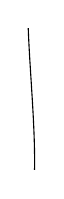
\begin{tikzpicture}[baseline=(current bounding box.north)]
\draw (0,0) .. controls (0.02,-0.55) and (0.09,-1.25) .. (0.08,-1.8);
\end{tikzpicture}
\end{minipage}%
\begin{minipage}[t]{0.965\linewidth}
\uline{Prop} Dans cet accouplement, $D(\unsure{M'_n|M_n})$ est orthogonal à ${}_nG'$, \deleted{\unsure{et}} (a un sens si ${}_nM'=0$) et \deleted{$D(M_{\unsure{n}}$} ${}_nG$ est orth. à $D(M_n)$ (a un sens si $\unsure{'}\,{}_nM=0$). Les accouplements induits
\end{minipage}

\diagram{\begin{tikzcd}[
ampersand replacement=\&,column sep=small,row sep=small,
execute at end picture={
\draw[gray,line width=0.3pt]
([xshift=-8pt,yshift=-3pt]\tikzcdmatrixname-1-2.south west)
.. controls ([xshift=-8pt,yshift=15pt]\tikzcdmatrixname-1-2.north west)
and ([xshift=10pt,yshift=15pt]\tikzcdmatrixname-1-2.north east)
.. ([xshift=10pt,yshift=-2pt]\tikzcdmatrixname-1-2.south east)
.. controls ([xshift=10pt,yshift=-12pt]\tikzcdmatrixname-2-2.south east)
and ([xshift=-12pt,yshift=-12pt]\tikzcdmatrixname-3-4.south west)
.. ([xshift=-3pt,yshift=-10pt]\tikzcdmatrixname-3-4.south);
}]
\deleted{\unsure{{}_nA/{}_n}} \& {}_nA'/{}_nG' \& \times \& D(M'_n)\arrow[rr] \& \& G_m\\
\& \unsure{\wr|\rho} \& \& \Vert \& \&\\
\& \unsure{,}\quad M'_n \& \& {}_n\unsure{T'|T} \& \&
\end{tikzcd}}

et
\diagram{\begin{tikzcd}[ampersand replacement=\&,column sep=small,row sep=small]
D(M_n) \& \times \& {}_nA/{}_nG\arrow[r,no head] \& G_m\\
\Vert \& \& \unsure{\wr|\rho} \&\\
{}_nT \& \& M_n \&
\end{tikzcd}},

ainsi que

\noindent\deleted{\unsure{et}}\quad
\begin{minipage}{0.85\linewidth}
\diagram{\begin{tikzcd}[ampersand replacement=\&,column sep=small,row sep=small]
{}_nG/{}_n\unsure{T|\Pi} \& \times \& {}_nG'/{}_nT'\\
\unsure{\Vert|\wr}\ \deleted{\unsure{{}_nT_n|{}_nT}} \& \& \unsure{\rho|\wr}\\
{}_n\unsure{\underline{B}|B} \& \& {}_nB'
\end{tikzcd}}
\end{minipage}

sont ceux qu'on devine.

\par\noindent
\begin{minipage}[t]{0.025\linewidth}
\vspace{1.2\baselineskip}
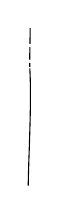
\begin{tikzpicture}[baseline=(current bounding box.north)]
\draw (0,0)--(-0.003,-0.20);
\draw (-0.004,-0.24)--(-0.006,-0.40);
\draw (-0.006,-0.44)--(-0.005,-0.49);
\draw (-0.005,-0.51) .. controls (0.02,-0.95) and (-0.02,-1.6) .. (-0.025,-2.0);
\end{tikzpicture}
\end{minipage}%
\begin{minipage}[t]{0.965\linewidth}
\uline{Corollaire} Si l'accouplement entre ${}_nB$ et ${}_nB'$ est une dualité parfaite \unsure{car|(car} $\unsure{\alpha|n}T_n=\unsure{n|\alpha}T'_n=0$) \deleted{\unsure{donc}} et si ${}_nM=0$, ${}_nM'=\unsure{0}$, $nB=B$, $\unsure{n|\mathbin{-}}B'=B'$, alors l'accouplement de ${}_nA$ et ${}_nA'$ est une dualité parfaite.
\end{minipage}
\margin{32}
